\documentclass[tikz,border=8pt]{standalone}
\usepackage{amsmath}
\usetikzlibrary{arrows.meta}
\begin{document}
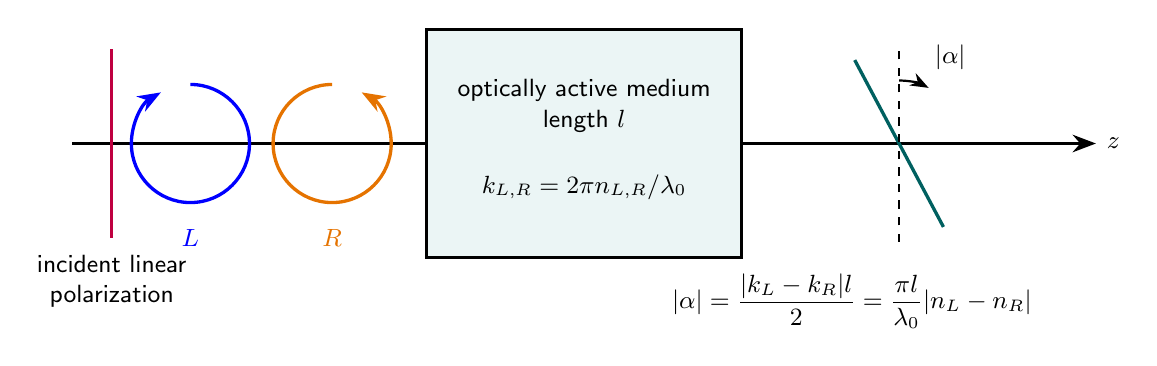
\begin{tikzpicture}[font=\sffamily\small,>=Stealth,thick]
  \draw[->,very thick] (-.5,0)--(12.5,0) node[right] {$z$};
  \draw[purple,very thick] (0,-1.2)--(0,1.2);
  \node[align=center] at (0,-1.75) {incident linear\\polarization};
  \draw[->,blue,very thick] (1,.75) arc[start angle=90,end angle=-240,radius=.75];
  \draw[->,orange!90!black,very thick] (2.8,.75) arc[start angle=90,end angle=420,radius=.75];
  \node[blue] at (1,-1.2) {$L$}; \node[orange!90!black] at (2.8,-1.2) {$R$};
  \fill[teal!8] (4,-1.45) rectangle (8,1.45);
  \draw[very thick] (4,-1.45) rectangle (8,1.45);
  \node[align=center] at (6,.48) {optically active medium\\length $l$};
  \node at (6,-.55) {$k_{L,R}=2\pi n_{L,R}/\lambda_0$};
  \draw[teal!75!black,very thick,rotate around={28:(10,0)}] (10,-1.2)--(10,1.2);
  \draw[dashed] (10,-1.25)--(10,1.25);
  \draw[->] (10,.8) arc[start angle=90,end angle=62,radius=.8];
  \node at (10.65,1.1) {$|\alpha|$};
  \node[align=center] at (9.4,-2)
    {$\displaystyle |\alpha|=\frac{|k_L-k_R|l}{2}
      =\frac{\pi l}{\lambda_0}|n_L-n_R|$};
\end{tikzpicture}
\end{document}
